\section*{Supplementary figures and tables}
\noindent\emph{Referenced from the main text; numbering matches the in-text references.}

\begin{table*}[t]\centering\setcounter{table}{0}\caption{Matched-stroke E-warp ratios across scenes, trajectories and detectors.}\label{tab:1}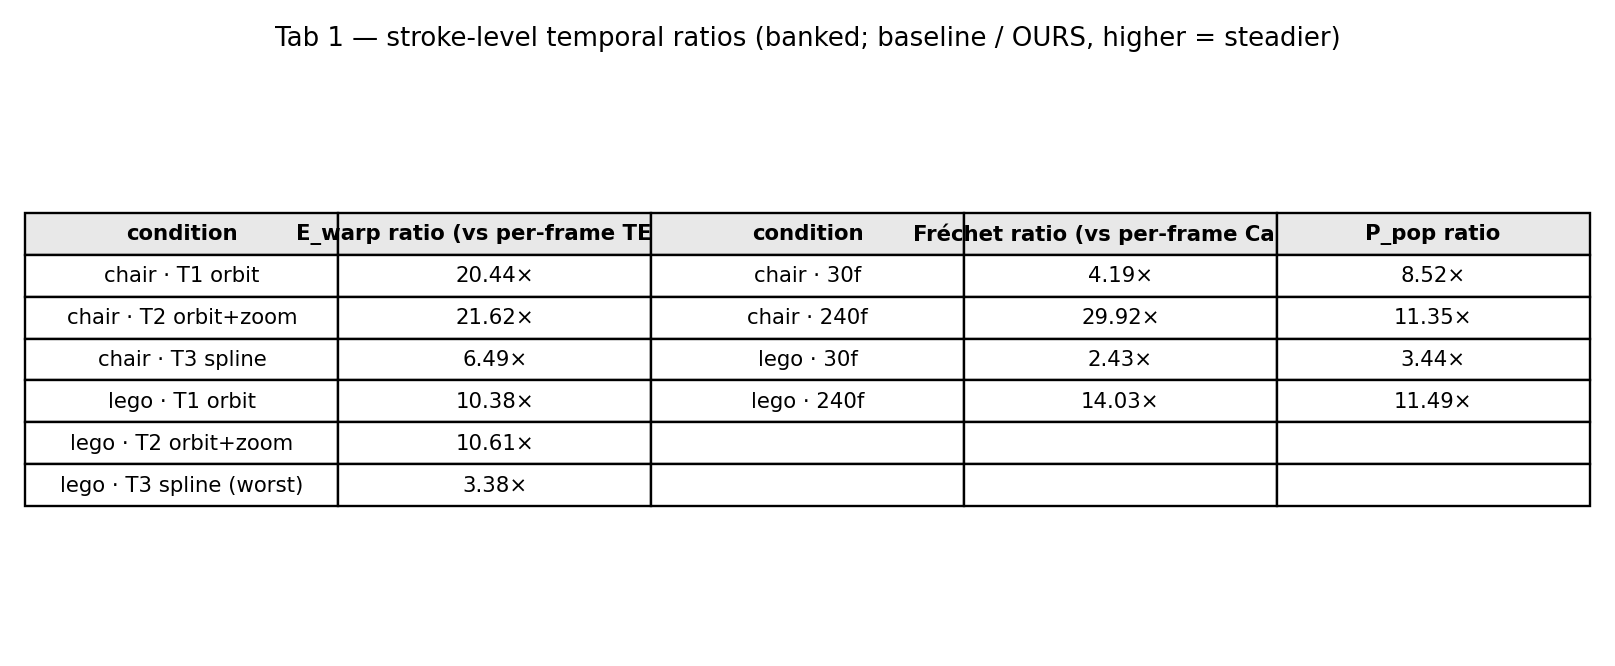
\includegraphics[width=0.8\textwidth]{assets/tab1_stroke_ratios.png}\end{table*}
\begin{table*}[t]\centering\setcounter{table}{1}\caption{Floor anatomy of the pooled-mean statistic.}\label{tab:2}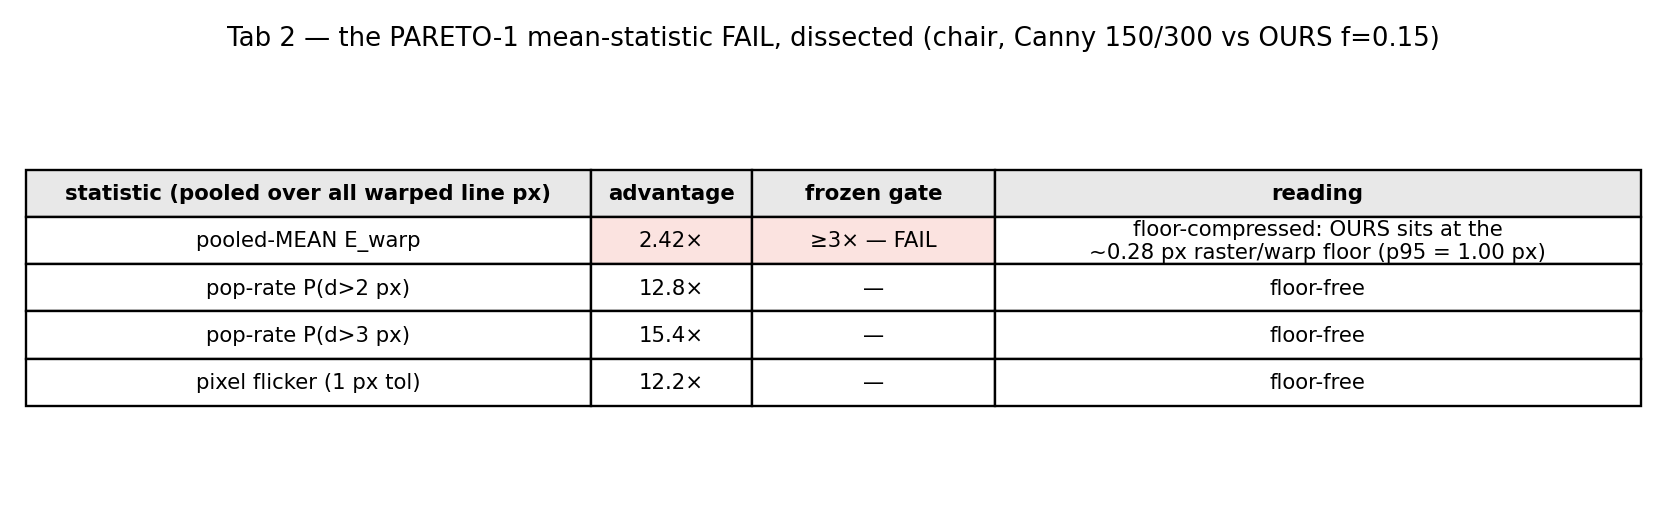
\includegraphics[width=0.62\textwidth]{assets/tab2_floor_anatomy.png}\end{table*}
\begin{table*}[t]\centering\setcounter{table}{2}\caption{K\textsubscript{geom}: geometric cues on the miss-set.}\label{tab:3}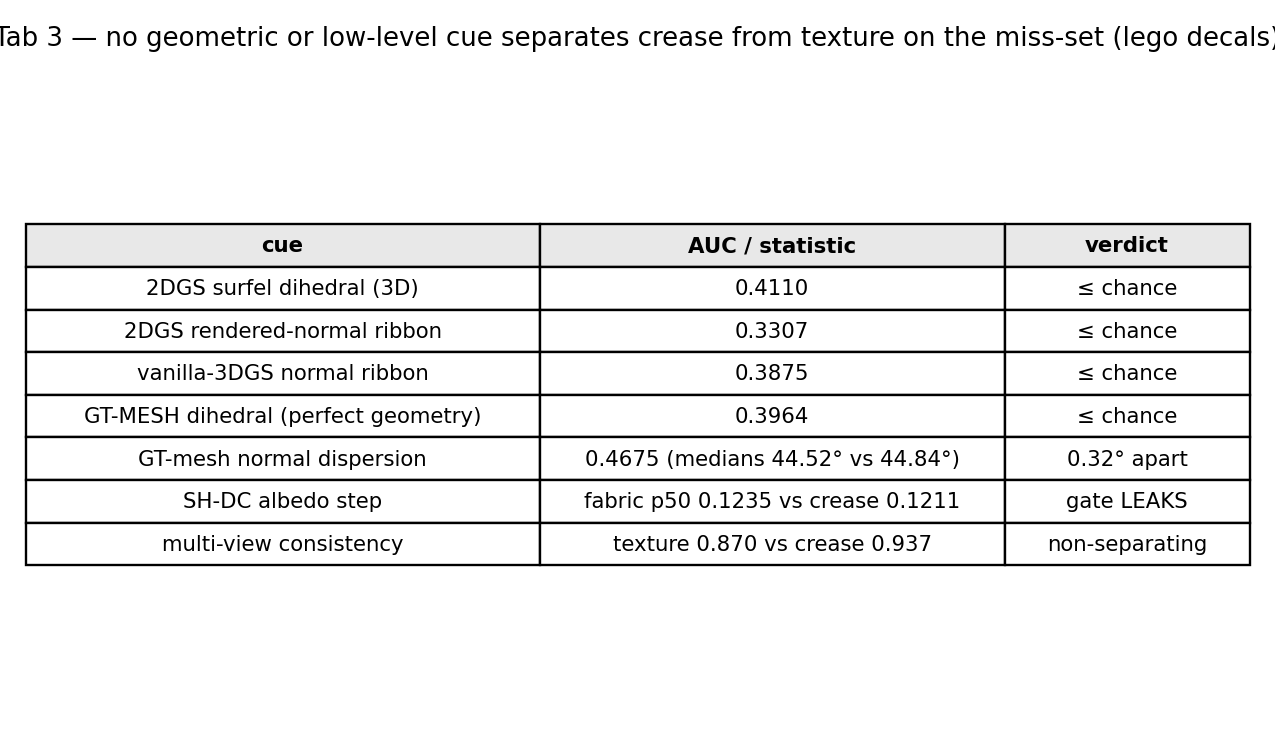
\includegraphics[width=0.55\textwidth]{assets/tab3_kgeom.png}\end{table*}
\begin{table*}[t]\centering\setcounter{table}{3}\caption{The frozen-gate ledger: every pre-registered gate, its bar, its measured value, and its disposition.}\label{tab:4}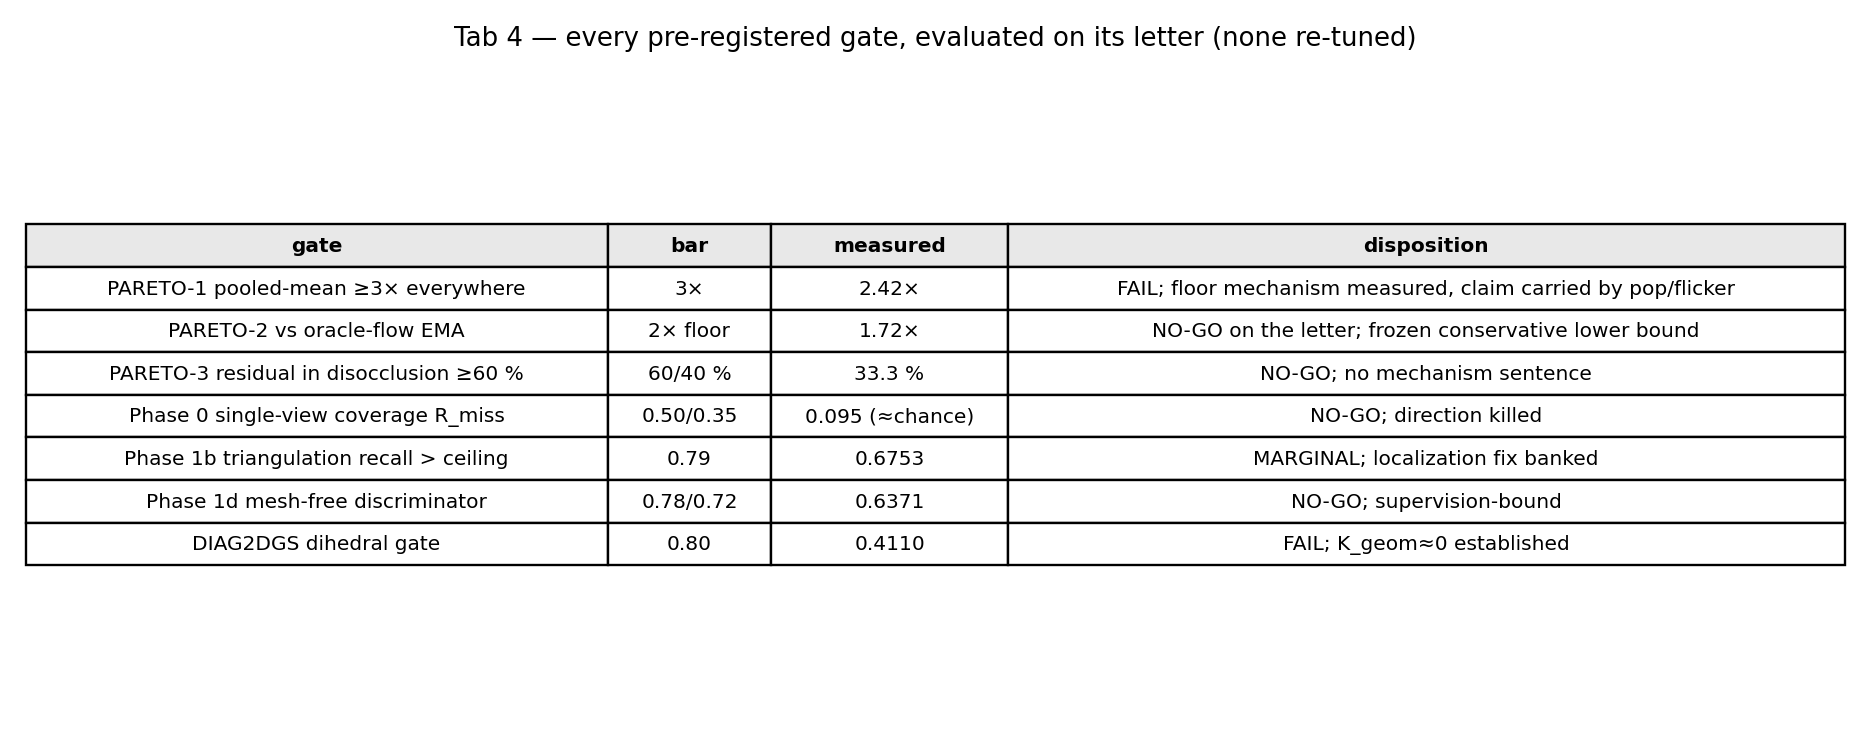
\includegraphics[width=0.62\textwidth]{assets/tab4_gate_ledger.png}\end{table*}
\begin{figure*}[t]\centering\setcounter{figure}{3}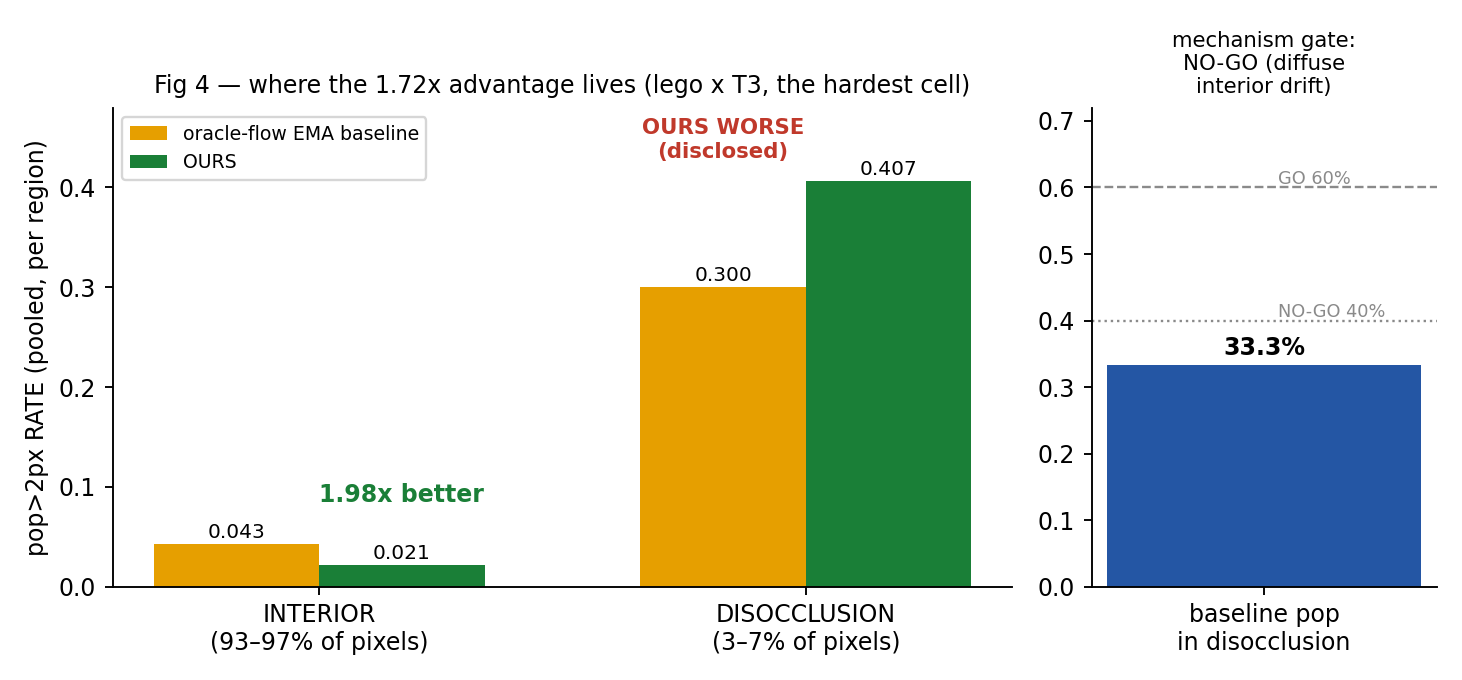
\includegraphics[width=0.75\textwidth]{assets/fig4_pareto3.png}\caption{Disocclusion decomposition of the hardest cell: the advantage is interior, reverses inside disocclusion regions, and the mechanism gate lands NO-GO.}\label{fig:4}\end{figure*}
\begin{figure*}[t]\centering\setcounter{figure}{6}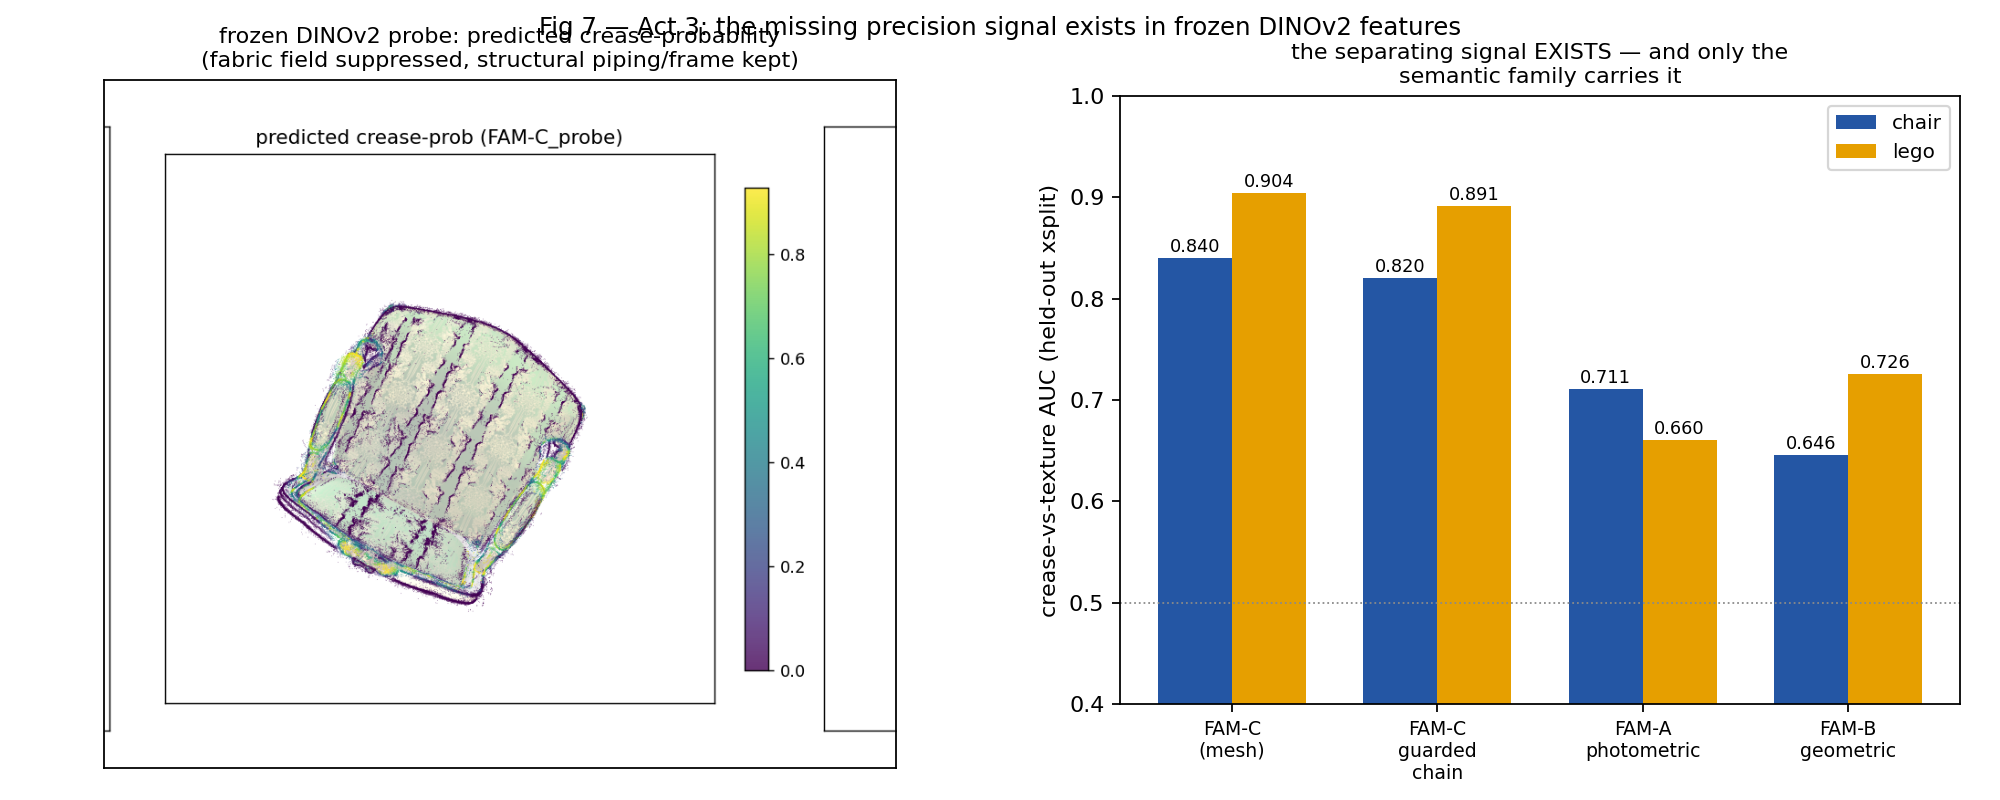
\includegraphics[width=0.85\textwidth]{assets/fig7_semantic.png}\caption{Act 3: frozen-DINOv2 crease-probability read-out and probe AUCs.}\label{fig:7}\end{figure*}
\begin{figure*}[t]\centering\setcounter{figure}{7}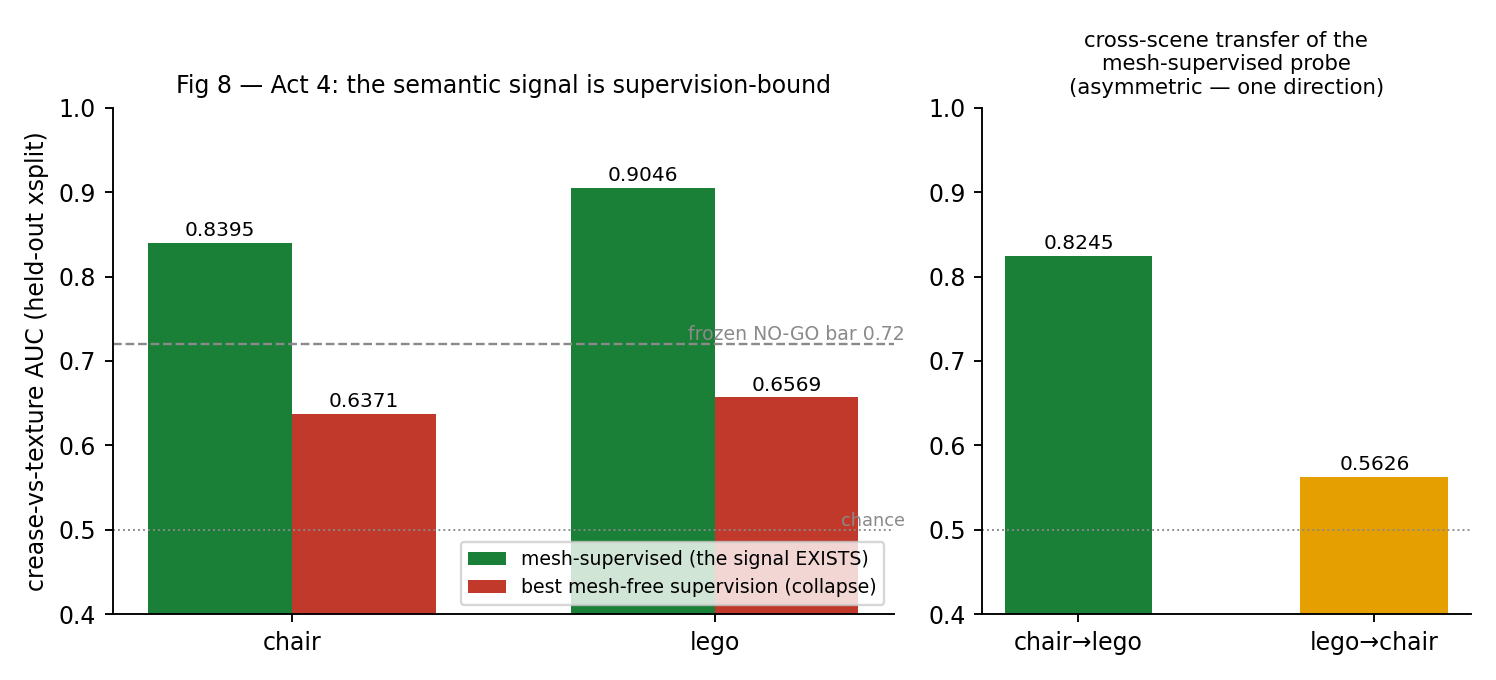
\includegraphics[width=0.75\textwidth]{assets/fig8_supervision.png}\caption{Act 4: the mesh-free supervision collapse, and the asymmetric cross-scene transfer. The mesh-supervised bars show the ceilings as recomputed in the falsification study; they agree with Act 3's split values quoted in the text to the third decimal.}\label{fig:8}\end{figure*}
\begin{figure*}[t]\centering\setcounter{figure}{8}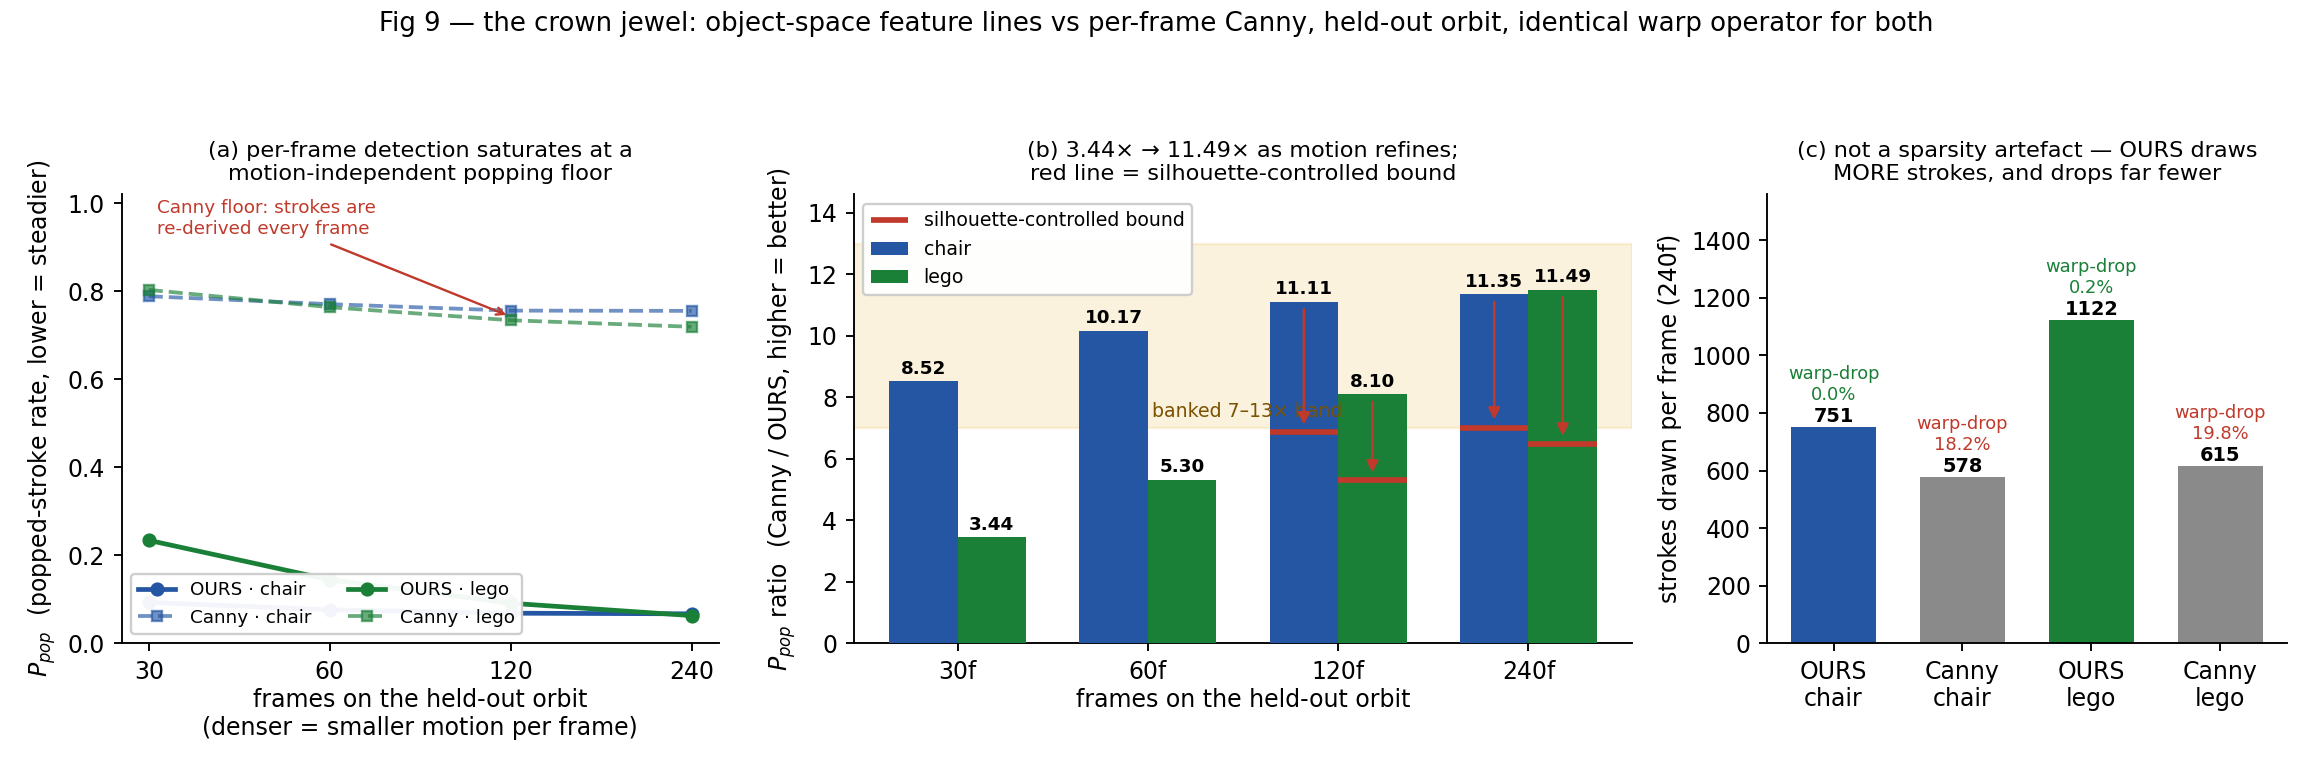
\includegraphics[width=0.98\textwidth]{assets/fig9_crownjewel.png}\caption{Object-space feature lines versus per-frame Canny on a held-out orbit, under an identical forward-warp operator for both pipelines. Left: per-frame detection saturates at a motion-independent popping floor while object-space strokes fall in proportion to the per-frame motion. Centre: the popping-rate ratio over the frame sweep, with the silhouette-controlled bound marked in red. Right: both confounds controlled --- the object-space pipeline draws more strokes per frame, not fewer, and almost none of them fail to warp.}\label{fig:9}\end{figure*}
\begin{table*}[t]\centering\setcounter{table}{4}\caption{Per-scene held-out summary: segment-raster precision and recall, popping rate for both pipelines, and the popping and Fr\'echet ratios. ficus is excluded by scene scoping rather than omitted --- too little of its surface lies far enough from a silhouette for crease-versus-flat to be well posed --- and no ficus result was ever run.}\label{tab:5}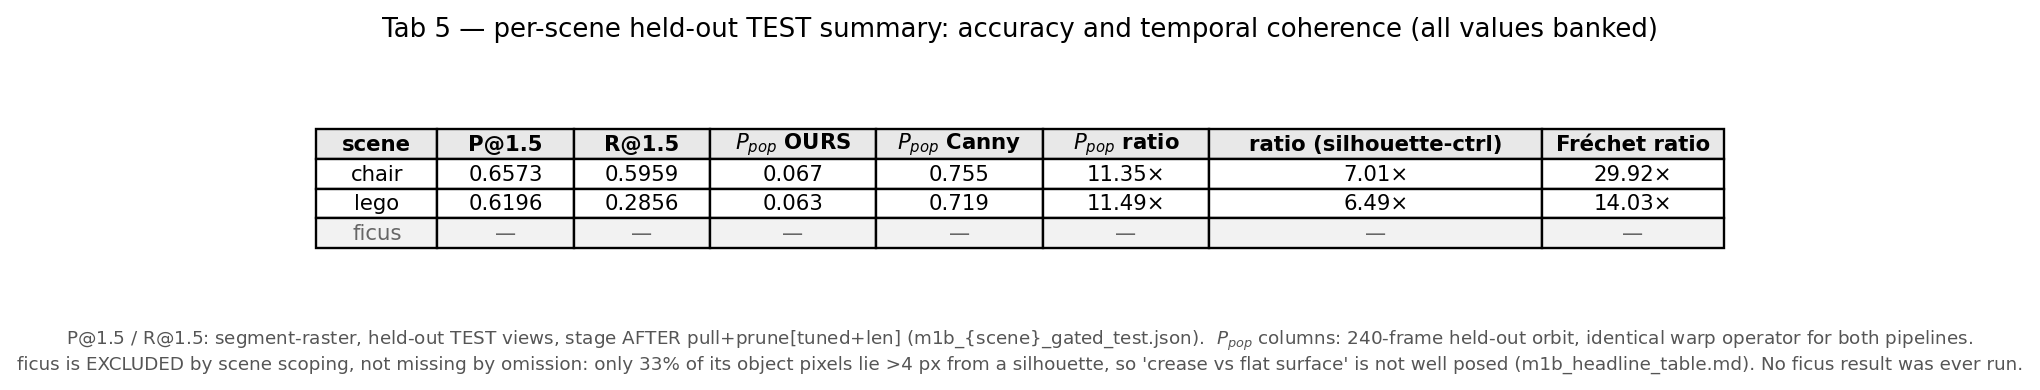
\includegraphics[width=0.82\textwidth]{assets/tab5_per_scene.png}\end{table*}
